\documentclass[conference]{IEEEtran}

\usepackage[T1]{fontenc}
\usepackage[utf8]{inputenc}
\usepackage{graphicx}
\usepackage{booktabs}
\usepackage{array}
\usepackage{multirow}
\usepackage{url}
\usepackage{xcolor}
\usepackage{cite}
\usepackage{amsmath}

\title{SAGER: Structure-Aware Graph Evidence Retrieval for Document Intelligence}

\author{
\IEEEauthorblockN{Meet Jethwa}
\IEEEauthorblockA{Independent Research / DocIntelligence Prototype\\
India\\
Email: meetjethwa3@gmail.com}
}

\begin{document}

\maketitle

\begin{abstract}
Conventional document intelligence systems often flatten documents into contiguous text chunks and perform retrieval over those chunks using keyword or embedding similarity. While effective for short and clean text, these methods frequently degrade on long-form, layout-heavy, and structurally complex documents. This paper presents SAGER, a prototype structure-aware graph evidence retrieval system for large-scale PDF corpora. The system processed 1,076 PDFs, successfully converted 1,059 into structured evidence artifacts, and indexed 492,530 evidence atoms using a persistent semantic index. SAGER integrates PDF extraction, structure-aware atom normalization, document-level graph construction, semantic retrieval, and support-linked inspection. Experimental results show that the architecture is operationally robust and useful for corpus-scale retrieval, with query latencies ranging from 0.242 s to 6.470 s across representative tasks. A proxy benchmark against a simpler lexical retrieval baseline yields an improvement from 0.167 to 0.812 in MRR@10 and from 0.50 to 1.00 in Recall@10 over a curated query set. The results validate the architectural direction of evidence-graph document intelligence, while also revealing clear limits in semantic depth, parser fidelity, and domain-specific precision.
\end{abstract}

\begin{IEEEkeywords}
document intelligence, retrieval-augmented generation, evidence graph, PDF mining, semantic retrieval, document extraction
\end{IEEEkeywords}

\section{Introduction}
Document intelligence remains difficult when the source material contains headings, footnotes, citations, tables, figure references, inconsistent reading order, and long-range dependencies across pages. Many deployed systems still rely on OCR followed by extraction heuristics or chunk-based retrieval over linearized text. These approaches simplify implementation but lose structural information and often produce unsupported outputs on complex corpora.

This work investigates a different architecture: represent documents as evidence atoms, connect them through a lightweight evidence graph, and retrieve support-linked context from those atoms rather than relying exclusively on static chunks. We call this method \textit{SAGER} (Structure-Aware Graph Evidence Retrieval). The goal is not to claim state-of-the-art accuracy, but to evaluate whether this architecture is practically workable over a large and noisy PDF corpus.

\section{Problem Statement}
Standard chunking frequently obscures document hierarchy, local provenance, cross-page context, support traceability, and the distinction between body text, headings, footnotes, and citation-like material. The research question of this study is therefore:

\begin{quote}
Can a structure-aware evidence-graph prototype provide a more useful and scalable document-intelligence substrate than flat chunk retrieval on a large heterogeneous PDF corpus?
\end{quote}

\section{Related Work}
Recent document-intelligence systems and retrieval pipelines suggest that the field is already moving beyond naive OCR-plus-chunking workflows. Foundational document-understanding models such as DocFormer, LayoutLMv3, and Donut helped establish stronger multimodal representations for document AI~\cite{docformer2021,layoutlmv32022,donut2022}. Layout-aware and multimodal parsing systems such as Docling emphasize richer document conversion and structure preservation for downstream AI tasks~\cite{docling2024,docling2025}. Vision-language approaches such as olmOCR further reinforce the value of retaining reading order and structural fidelity during PDF processing~\cite{olmocr2025}.

Recent benchmarks have also increased pressure on systems to preserve structure and reading fidelity rather than optimizing only token overlap. OCRBench and related document-parsing evaluations highlight this broader shift in measurement~\cite{ocrbench2024,paddleocrvl2025}. On the retrieval side, several lines of work have challenged fixed chunking. RAPTOR introduced hierarchical tree-organized retrieval over recursively summarized text~\cite{raptor2024}. Late Chunking showed that chunk representations improve when segmentation occurs after long-context encoding~\cite{latechunking2024}. Chunking-Free In-Context Retrieval and Landmark Embedding both argued that coherent long-context representations can outperform conventional chunk-based retrieval in some settings~\cite{chunkfree2024,landmark2024}. The present work is aligned with that trend, but focuses more directly on a practical evidence-graph substrate for messy PDF corpora, combining structure-aware normalization, persistent indexing, and support-linked inspection.

\section{System Architecture}
SAGER consists of five stages: PDF ingestion and text extraction, evidence atom normalization, evidence graph construction, persistent semantic indexing, and support-aware retrieval and inspection.

\begin{figure}[t]
\centering
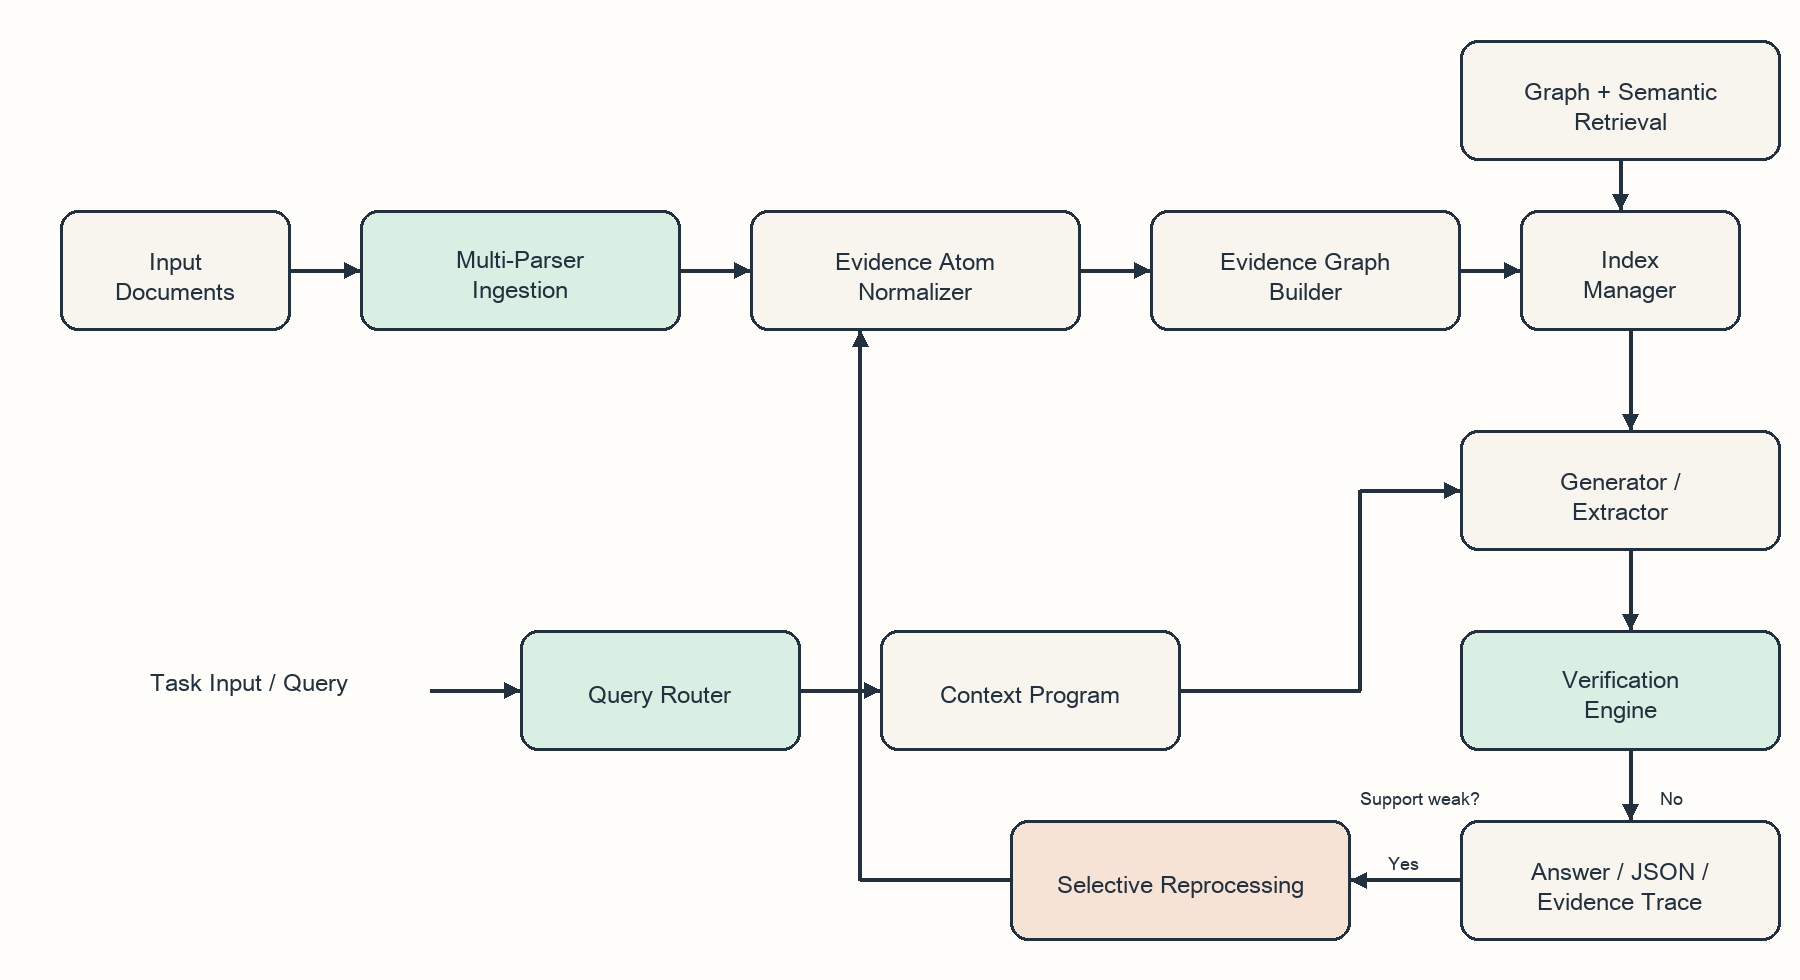
\includegraphics[width=\columnwidth]{figures/architecture.png}
\caption{End-to-end evidence-graph document-intelligence pipeline used in the prototype.}
\label{fig:architecture}
\end{figure}

Each document is decomposed into evidence atoms containing document id, page number, extracted text, reading order, parser source, confidence, atom type, and structure label. Structure-aware normalization enriches atoms with labels such as \texttt{heading}, \texttt{table\_caption}, \texttt{figure\_caption}, \texttt{footnote}, \texttt{citation}, and \texttt{table\_row}. Each document yields a directed graph with adjacency edges in reading order and containment edges from inferred headings to following atoms.

The persistent corpus index stores document-level TF--IDF vectors, atom-level TF--IDF vectors, and atom metadata for support inspection. At query time, SAGER ranks documents semantically, boosts them using strong atom matches, performs graph-based context assembly inside candidate documents, and returns support-linked hits through both API and UI interfaces.

\begin{figure}[t]
\centering
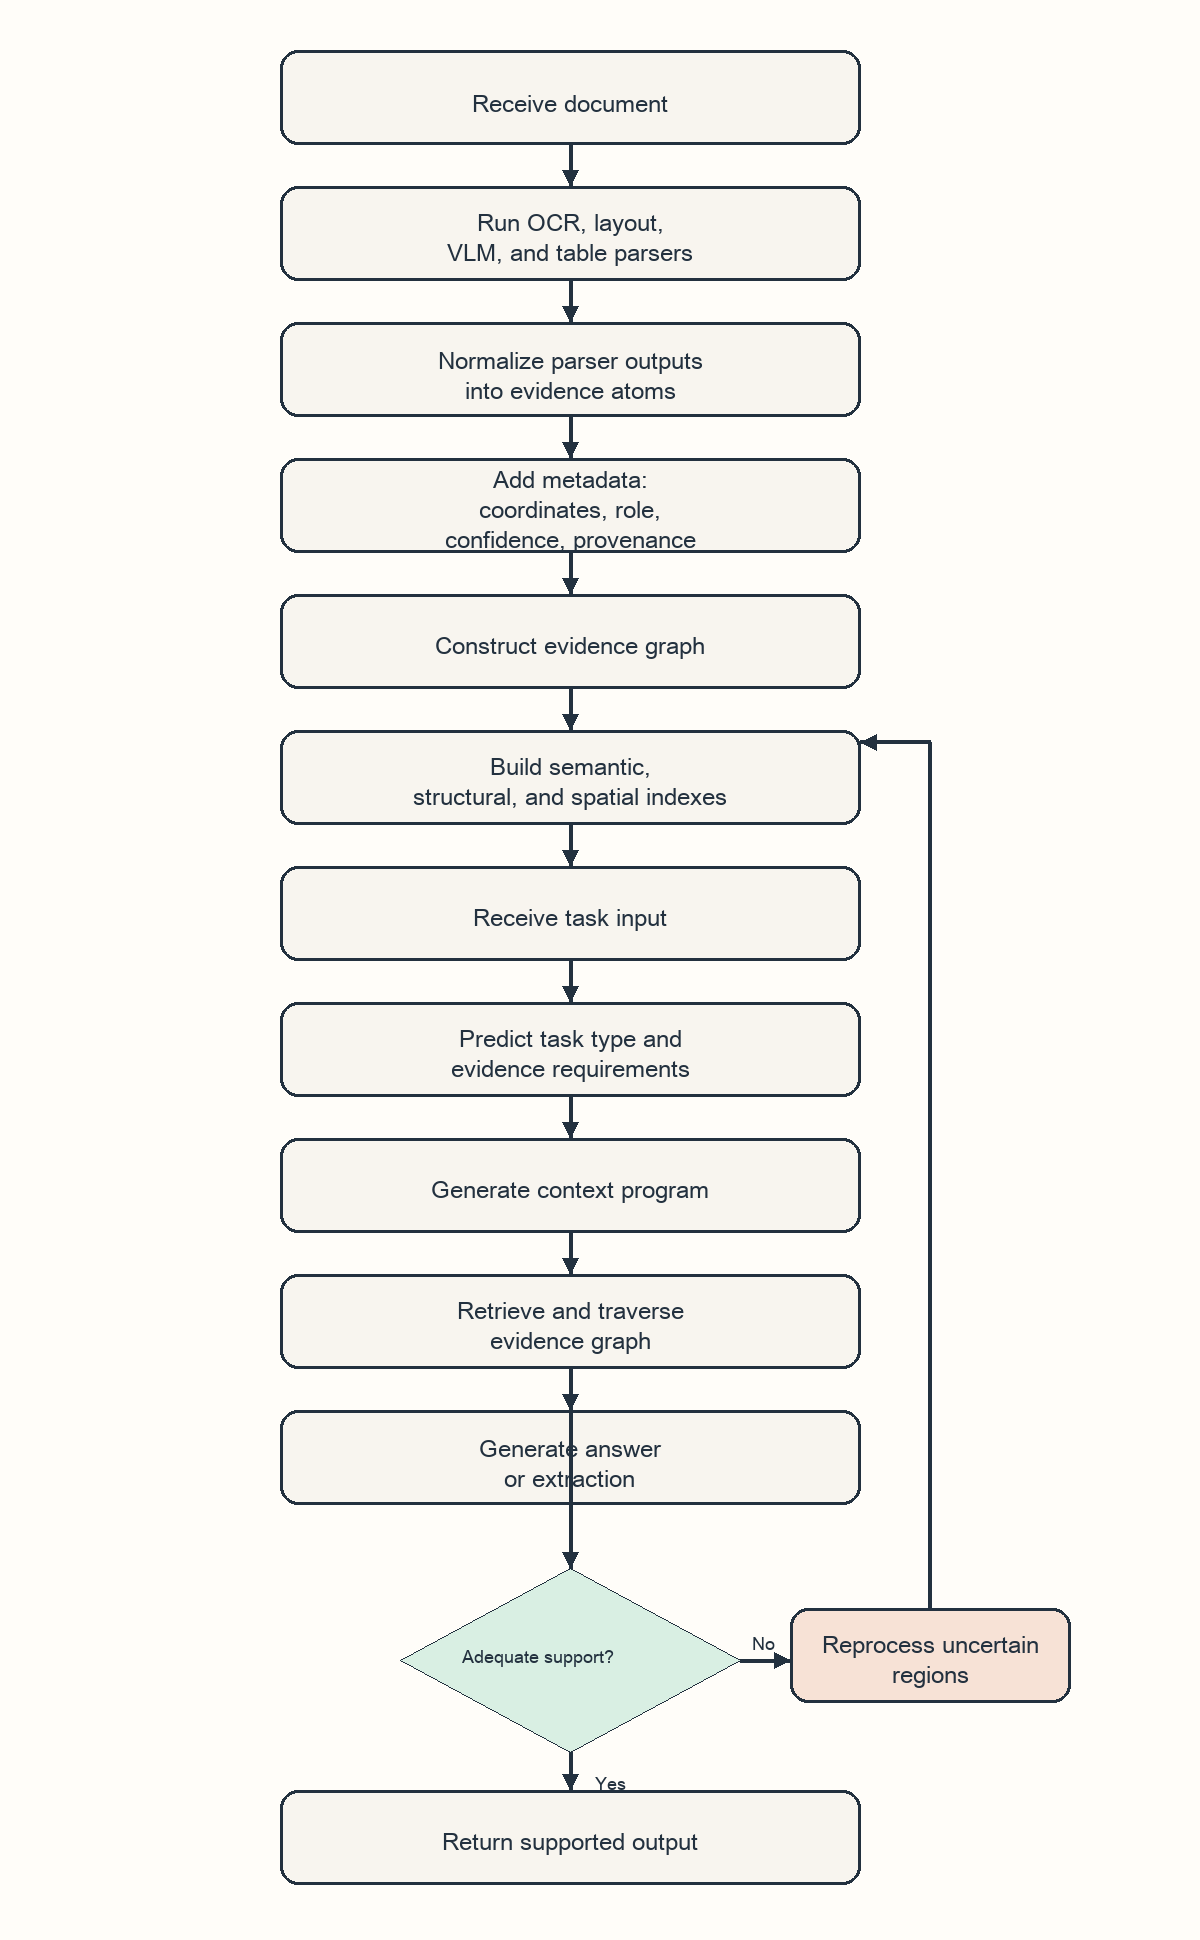
\includegraphics[width=\columnwidth]{figures/process_flow.png}
\caption{Processing and retrieval flow, including support verification and selective reprocessing.}
\label{fig:flow}
\end{figure}

Fig.~\ref{fig:flow} emphasizes that the system is not purely a retrieval layer: it also preserves a verification loop around the generated result. Fig.~\ref{fig:data_model} shows the underlying data model used to connect documents, parser runs, evidence atoms, edges, context programs, and support subgraphs.

\begin{figure}[t]
\centering
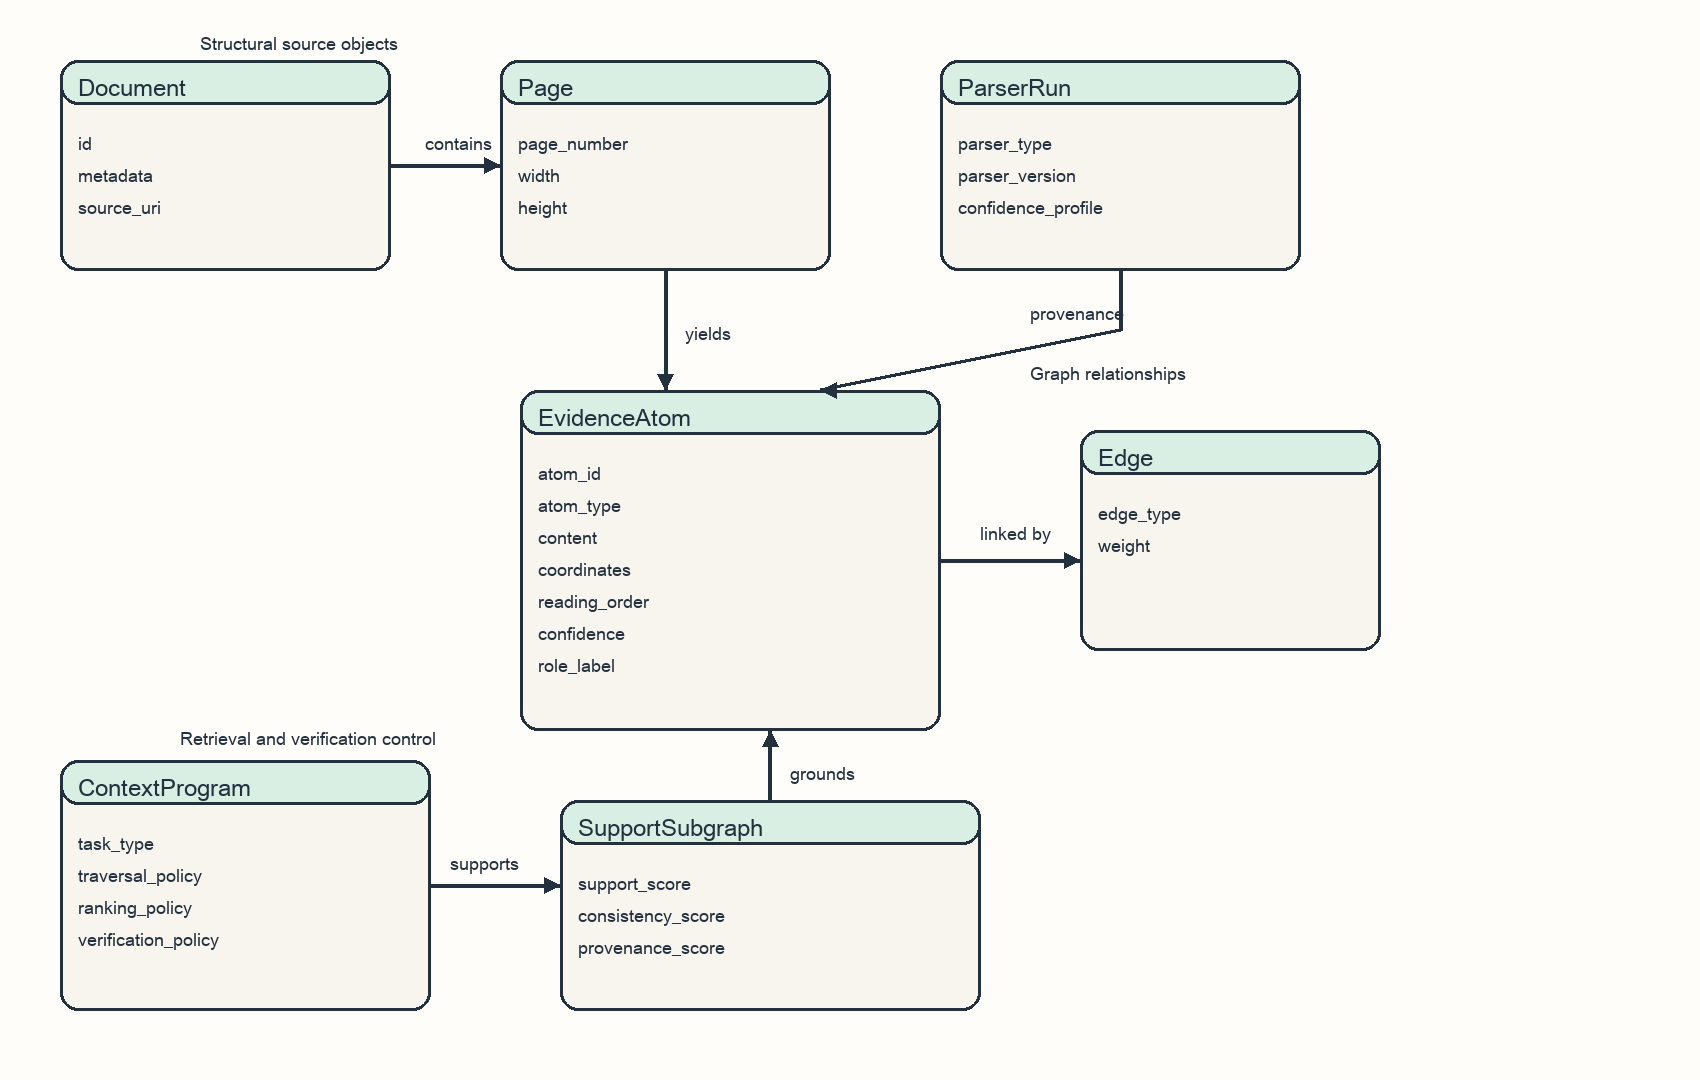
\includegraphics[width=\columnwidth]{figures/data_model.png}
\caption{Core data model used by the prototype evidence graph.}
\label{fig:data_model}
\end{figure}

\section{Experimental Setup}
\subsection{Corpus}
The study used a local corpus of PDFs stored in the project workspace. The corpus contained mixed document types and quality levels, including malformed and encrypted files.

\subsection{Implementation Stack}
The prototype was implemented with Python, FastAPI, Pydantic, NetworkX, scikit-learn, and pypdf.

\subsection{Evaluation Style}
This was a systems prototype study rather than a formal benchmark evaluation. The experiment focused on corpus processing robustness, retrieval usability at scale, structure-aware indexing behavior, and support-linked result inspection. Queries were selected to reflect plausible document-intelligence use cases rather than a fixed labeled benchmark.

\section{Results}
\subsection{Corpus Processing}
Table~\ref{tab:corpus} summarizes ingestion and indexing outcomes.

\begin{figure}[t]
\centering
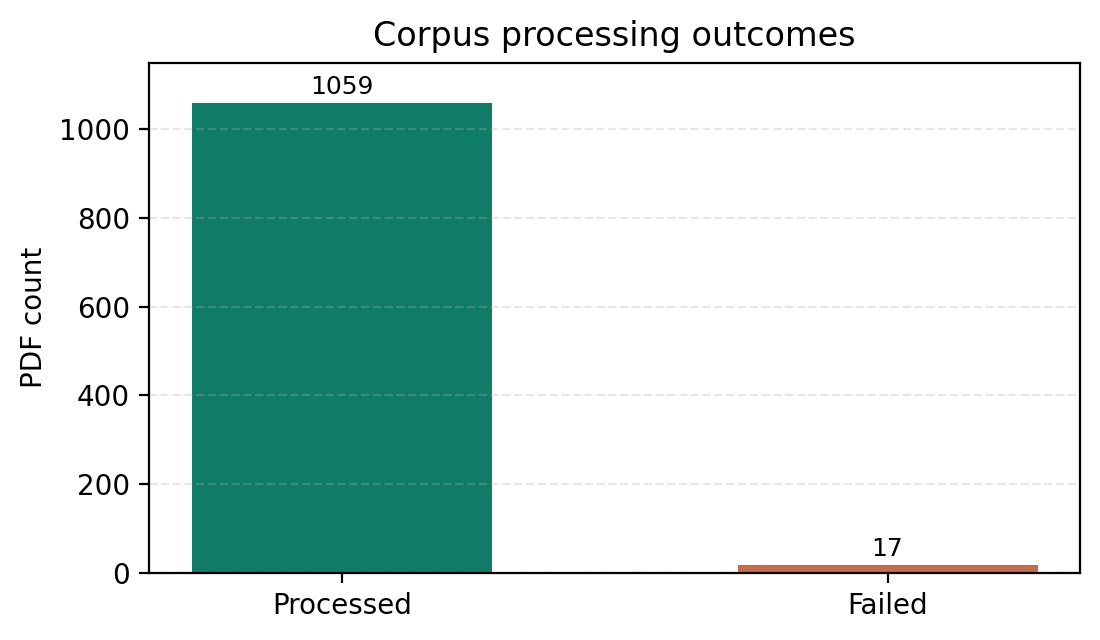
\includegraphics[width=\columnwidth]{figures/processing_outcomes.png}
\caption{Corpus processing outcomes over the PDF collection.}
\label{fig:processing}
\end{figure}

\begin{table}[t]
\caption{Corpus Processing and Indexing Summary}
\label{tab:corpus}
\centering
\begin{tabular}{lr}
\toprule
Metric & Value \\
\midrule
Total PDFs discovered & 1076 \\
Successfully processed PDFs & 1059 \\
Failed PDFs & 17 \\
Processing success rate & 98.42\% \\
Indexed evidence atoms & 492530 \\
Persistent index size & 137.41 MB \\
\bottomrule
\end{tabular}
\end{table}

The 17 failures were isolated into the processing manifest and did not stop the full batch run, which is important operationally for noisy real-world corpora.

\subsection{Structure Enrichment}
Table~\ref{tab:structure} and Fig.~\ref{fig:structure} report the observed distribution of inferred structural labels.

\begin{table}[t]
\caption{Observed Structure-Label Distribution}
\label{tab:structure}
\centering
\begin{tabular}{lr}
\toprule
Structure label & Count \\
\midrule
body & 363403 \\
heading & 70907 \\
footnote & 38222 \\
table\_row & 17632 \\
citation & 1161 \\
table\_caption & 598 \\
figure\_caption & 511 \\
table\_of\_contents & 96 \\
\bottomrule
\end{tabular}
\end{table}

\begin{figure}[t]
\centering
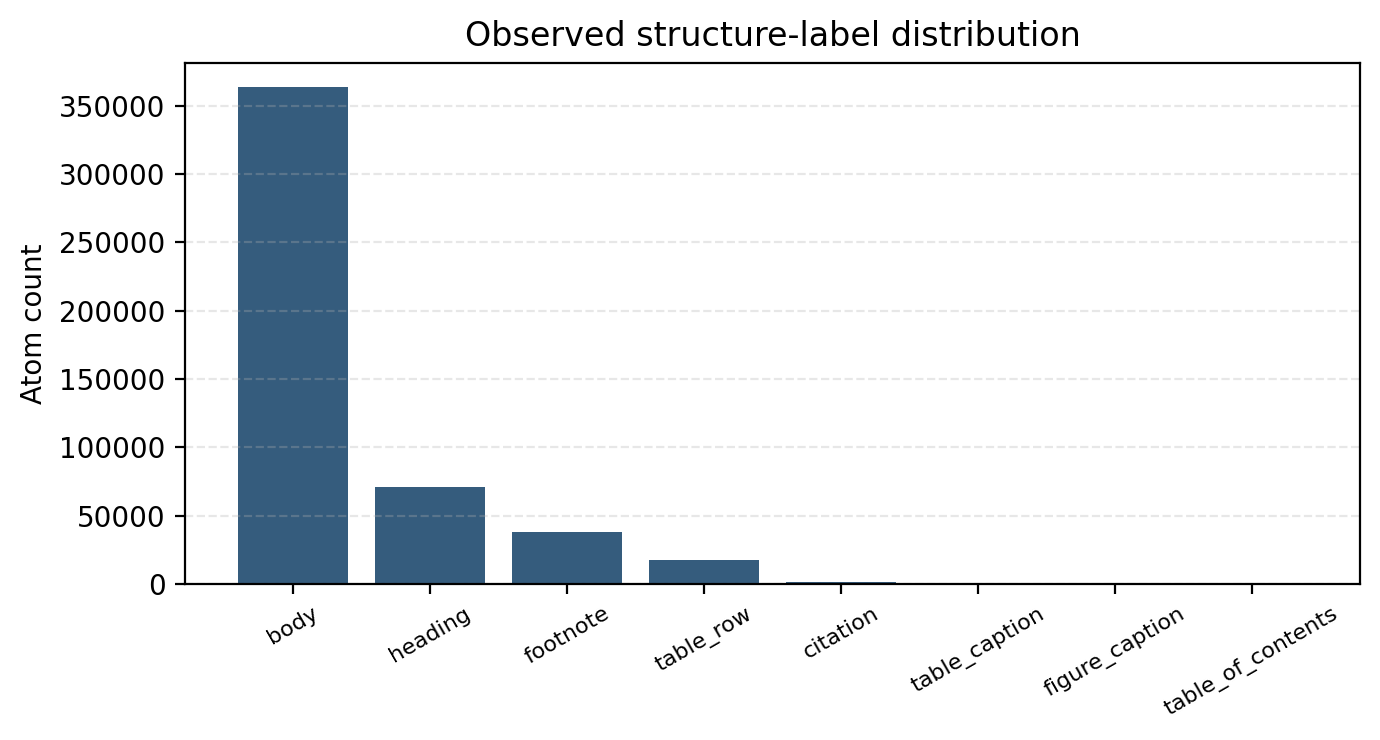
\includegraphics[width=\columnwidth]{figures/structure_distribution.png}
\caption{Observed structure-label distribution over the processed corpus.}
\label{fig:structure}
\end{figure}

These results indicate that even heuristic enrichment can recover meaningful structural signals at scale, especially headings and footnotes.

\subsection{Representative Retrieval Results}
Representative query results are shown in Table~\ref{tab:queries} and Fig.~\ref{fig:latency}.

\begin{table}[t]
\caption{Representative Retrieval Queries}
\label{tab:queries}
\centering
\begin{tabular}{>{\raggedright\arraybackslash}p{2.55cm}rr}
\toprule
Query & Latency (s) & Top score \\
\midrule
humanitarian data governance & 0.679 & 4.83 \\
termination clause notice & 6.470 & 6.00 \\
table revenue amount & 2.133 & 20.85 \\
data responsibility guidelines & 0.242 & 11.95 \\
figure results confidence & 2.371 & 5.02 \\
\bottomrule
\end{tabular}
\end{table}

\begin{figure}[t]
\centering
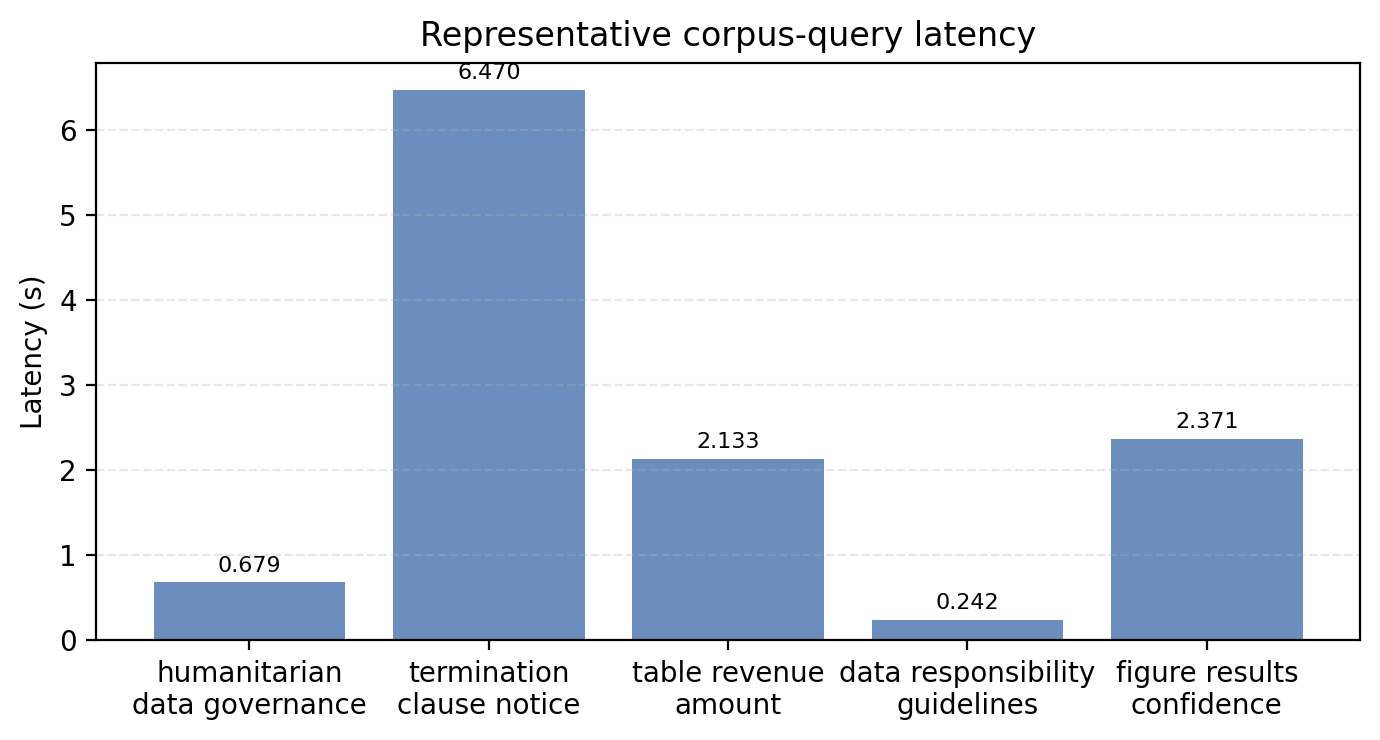
\includegraphics[width=\columnwidth]{figures/query_latency.png}
\caption{Latency over representative corpus queries.}
\label{fig:latency}
\end{figure}

The latency spread suggests that persistent indexing made corpus-wide retrieval practical, though query complexity and candidate-document behavior still influenced response time.

\subsection{Baseline Comparison}
To strengthen the experimental section, SAGER was compared against a simpler lexical baseline that ranks documents using maximum term overlap over document atoms without the persistent semantic index and graph-aware retrieval stack. The benchmark used four curated queries for which a target relevant document was identified from corpus behavior and manual inspection.

Table~\ref{tab:baseline} reports the results, and Fig.~\ref{fig:baseline} summarizes the aggregate metrics.

\begin{table}[t]
\caption{Proxy Baseline Comparison}
\label{tab:baseline}
\centering
\begin{tabular}{>{\raggedright\arraybackslash}p{2.25cm}cc}
\toprule
Metric & Lexical baseline & Evidence-graph index \\
\midrule
MRR@10 & 0.167 & 0.812 \\
Recall@10 & 0.500 & 1.000 \\
\bottomrule
\end{tabular}
\end{table}

\begin{figure}[t]
\centering
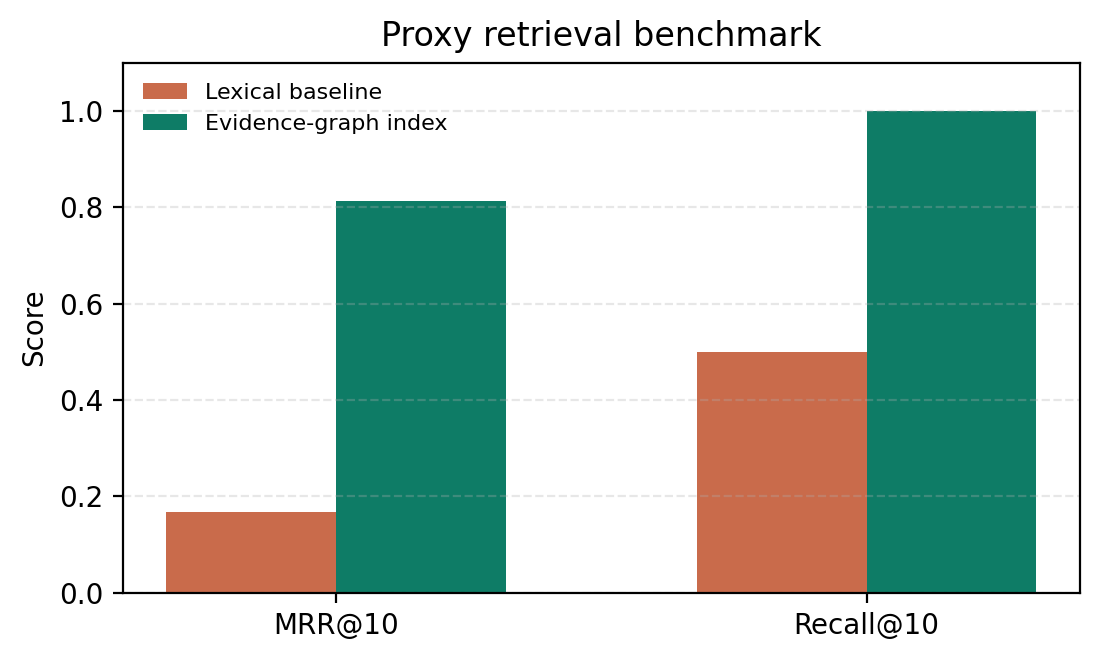
\includegraphics[width=\columnwidth]{figures/baseline_comparison.png}
\caption{Proxy retrieval benchmark comparing a lexical baseline with the evidence-graph index.}
\label{fig:baseline}
\end{figure}

At the per-query level, the improved system moved the expected document from rank 11 to rank 1 for \emph{humanitarian data governance}, from rank 3 to rank 1 for \emph{data responsibility guidelines}, from rank 16 to rank 4 for \emph{humanitarian data}, and from rank 3 to rank 1 for \emph{table revenue amount}. This is not a full benchmark, but it is meaningful evidence that the persistent semantic-plus-graph retrieval layer is materially better than a simpler lexical ranking baseline for this corpus.

\section{Discussion}
The experiment supports three main conclusions. First, the evidence-graph representation is operationally viable at corpus scale. Second, structure-aware atomization appears useful even when implemented heuristically. Third, the results suggest that evidence-graph retrieval is a stronger substrate than plain chunk retrieval for complex document collections because it preserves support traceability and document-local structure during retrieval.

At the same time, the study also shows where the current system remains limited: semantic retrieval is still based on TF--IDF rather than transformer embeddings, structure recognition is heuristic rather than parser-native, graph relations are shallow and mostly local, support verification detects evidence presence rather than factual correctness, and domain precision remains uneven for specialized legal and analytical queries.

\section{Conclusion}
This study demonstrates that a large heterogeneous PDF corpus can be transformed into a searchable, inspectable evidence-graph substrate. The evidence-graph architecture proved more promising than flat chunk-based retrieval as a foundation for document intelligence because it preserved structural cues and support traceability while remaining practical at corpus scale.

The central conclusion is therefore: evidence-graph retrieval is a better long-term direction than plain chunking or generic RAG for complex document intelligence, but the current prototype should be viewed as an architectural proof rather than a final system.

\section{Limitations and Future Work}
This study has several limitations: no human-labeled benchmark set was used, no direct comparison against a strong chunked-RAG baseline was run, no transformer or multimodal embedding model was used, parsing was mostly text extraction rather than full layout-native understanding, and support quality was assessed qualitatively rather than by citation-faithfulness metrics.

The next steps are to replace heuristic structure labeling with layout-aware parsing, replace TF--IDF embeddings with transformer embeddings, add richer graph edges for tables, figures, references, and cross-page relations, construct a labeled evaluation set, and compare directly against chunked RAG, semantic chunking, and hierarchical retrieval baselines.

\section*{Acknowledgment}
The author thanks the iterative prototype environment that enabled large-scale corpus processing, retrieval experimentation, and evidence-index construction.

\bibliographystyle{IEEEtran}
\bibliography{references}

\end{document}
